%! TEX root = main.tex  %
\documentclass[main.tex]{subfiles} % Wichtig!

\begin{document}


\subsection{Projektmanagement}

Das Projektmanagement spielt eine zentrale Rolle in der Vorbereitungsphase meiner Bachelorarbeit 
und bildet die Grundlage für den Erfolg des gesamten Vorhabens. Dabei geht es nicht nur um die 
reine Planung, sondern auch um eine effiziente Steuerung und kontinuierliche Kontrolle aller 
Arbeitspakete und derer Ergebnisse. Die besondere Herausforderung meiner Arbeit liegt darin, 
das umfangreiche Themengebiet, das für diese Bachelorarbeit relevant ist, innerhalb des engen 
Zeitrahmens von 14 Wochen sinnvoll und fundiert zu bearbeiten. Das Themengebiet umfasst diverse 
Bereiche der Informatik. Darunter fallen Audioverarbeitung, maschinelles Lernen, 
Softwareentwicklung und auch einiges an mathematischem Hintergrundwissen. Daher wurde ein agiles 
Vorgehensmodell gewählt. Dies bedeutet, dass sowohl die Planung als auch die Umsetzung in iterative 
Zyklen unterteilt sind. Während es zu Beginn eine grobe Struktur und Zielsetzung gibt, ermöglicht 
diese Herangehensweise Flexibilität in der Durchführung. Dadurch können Veränderungen oder 
unerwartete Ereignisse leichter integriert und die Bachelorarbeit fortlaufend optimiert werden.

\subsection{Grobplanung}
Die Grobplanung zeigt die wichtigsten Meilensteine des Projekts auf. Ausserdem werden die 
Themengebiete, die für die Bachelorarbeit relevant sind, aufgezeigt.

\begin{figure}[h]
    \hspace{-0.075\linewidth} % 15% divided by 2 to center the image
    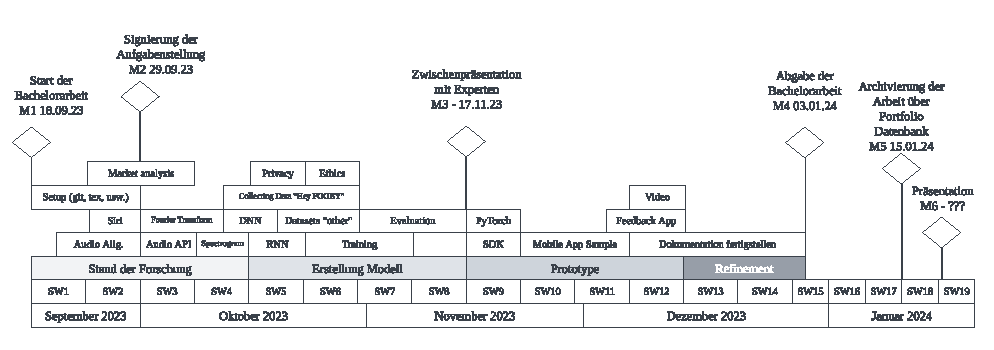
\includegraphics[width=1.15\linewidth]{img/projectplan.pdf}
    \caption{Grobplanung}
    \label{fig:grobplanung}
\end{figure}




\subsubsection{Produkt Backlog}

In der Vorbereitungsphase kann ein anfängliches Produkt Backlog als einfache Tabelle
dargestellt werden. Ein Beispiel für eine solche Tabelle ist in Abbildung 5 dargestellt.



\begin{figure}[h]
    \centering
    
\includegraphics[width=0.7\linewidth]{img/placeholder.png}
    \caption{Tabelle für das anfängliche Product Backlog}
    \label{fig:backlog_table}
\end{figure}


\subsubsection{Risikomanagement}
Risikomanagement dient dem Zweck, mögliche Probleme vorwegzunehmen. Die Verwendung von
Checklisten, Brainstorming mit den Anspruchsgruppen und die von Erfahrungen
aus früheren Projekten sind mögliche Strategien zur Identifikation möglicher Risiken.

\begin{table}[h]
    \centering
    \caption{Beispiel-Tabelle für Risikomanagement}
    \begin{tabular}{|c|c|c|}
        \hline
        Kopf 1 & Kopf 2 & Kopf 3 \\
        \hline
        Wert 1 & Wert 2 & Wert 3 \\
        \hline
        Wert 4 & Wert 5 & Wert 6 \\
        \hline
    \end{tabular}
    \caption{Eine einfache Tabelle}
    \label{tab:meineTabelle}

\end{table}



\end{document}

